\documentclass[11pt]{article}
\usepackage[margin=1in]{geometry}
\usepackage{amsmath,amssymb,amsthm}
\usepackage{graphicx}
\usepackage[hidelinks]{hyperref}

\newtheorem{theorem}{Theorem}
\newtheorem{lemma}{Lemma}

\newcommand{\NN}{\mathbb N}
\newcommand{\RR}{\mathbb R}

\begin{document}

\begin{center}
{\Large The nn-bounded operators are not closed under nn-convergence}\\[3pt]
{\large A counterexample to a question in arXiv:math/0004049}
\end{center}

\section*{Source Question}

Troitsky defines nn-convergence for operators on a topological vector
space and asks whether the class of nn-bounded operators is closed
relative to that convergence \cite{Troitsky}.

\begin{figure}[h]
\centering

\includegraphics[width=0.92\textwidth]{figures/open_problem_crop.png}
\caption{The definition of nn-convergence and the displayed question.}
\end{figure}

The source paper also records that the left shift on \(\RR^\NN\), with
the topology of coordinatewise convergence, is continuous but not
nn-bounded.

\begin{figure}[h]
\centering
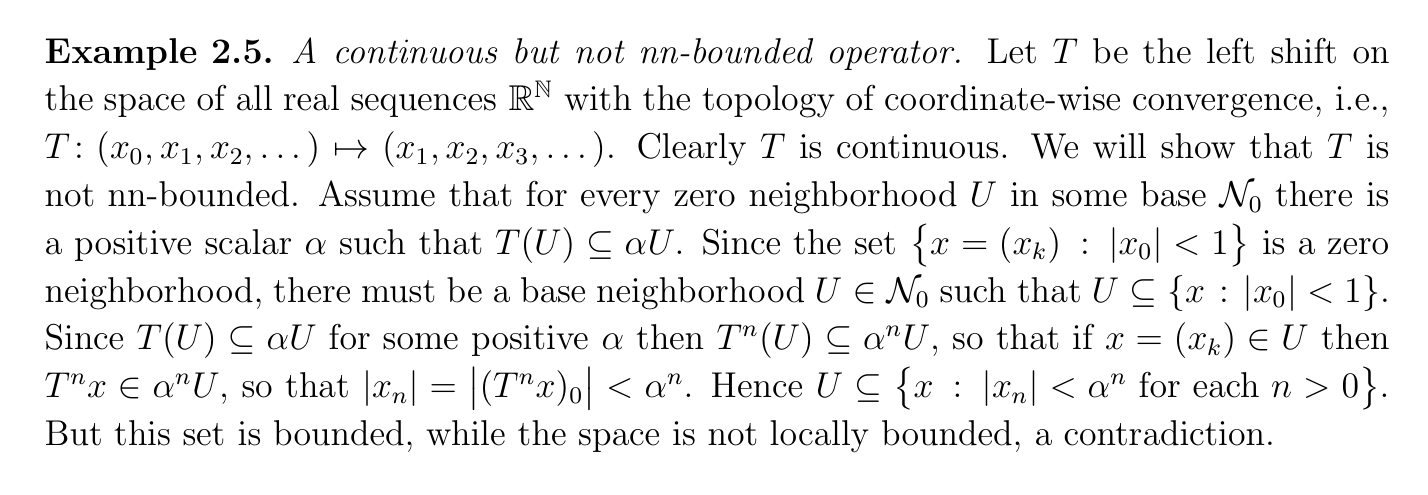
\includegraphics[width=0.92\textwidth]{figures/source_left_shift_crop.png}
\caption{Example 2.5 in the source paper.}
\end{figure}

\section*{Proof Intuition}

The topology of \(\RR^\NN\) only tests finitely many coordinates at a
time. Finite truncations of the left shift are harmless: each one has
finite-dimensional range, hence maps a suitable zero neighborhood into a
bounded set. But for any fixed finite coordinate test, a far enough
truncation agrees with the full left shift on all tested coordinates.
Thus the truncated shifts converge to the full left shift in
nn-convergence even though the full shift is not nn-bounded.

\section*{Counterexample}

\begin{theorem}
The class of nn-bounded operators need not be closed relative to
nn-convergence.
\end{theorem}

\begin{proof}
Let \(X=\RR^\NN\) with the product topology, where coordinates are
indexed by \(0,1,2,\ldots\). A basic zero neighborhood is a set
\[
  U(F,\delta)=\{x\in X: |x_j|<\delta_j \text{ for every } j\in F\},
\]
where \(F\subset\NN\) is finite and each \(\delta_j>0\). A subset of
\(X\) is bounded if and only if it is bounded in each coordinate.

Let \(L:X\to X\) be the left shift
\[
  L(x_0,x_1,x_2,\ldots)=(x_1,x_2,x_3,\ldots).
\]
For \(N\ge 0\), let \(P_N\) be the coordinate projection
\[
  P_N(y_0,y_1,\ldots)=(y_0,\ldots,y_N,0,0,\ldots),
\]
and put \(S_N=P_NL\). We first show that each \(S_N\) is nn-bounded. In
fact it is nb-bounded. The zero neighborhood
\[
  V_N=\{x\in X: |x_j|<1\text{ for }1\le j\le N+1\}
\]
is mapped by \(S_N\) into the set of all \(y\) satisfying
\(|y_j|<1\) for \(0\le j\le N\) and \(y_j=0\) for \(j>N\). This image is
coordinatewise bounded, hence bounded in \(X\). Thus \(S_N\) is
nb-bounded, and by the hierarchy in \cite[Proposition 2.1]{Troitsky},
each \(S_N\) is nn-bounded.

Now we prove that \(S_N\to L\) in nn-convergence. It is enough to use the
standard base \(U(F,\delta)\) above. Fix such a \(U=U(F,\delta)\) and
fix \(\varepsilon>0\). Choose \(N\ge \max F\), with the convention that
the condition is empty if \(F=\varnothing\). For \(j\in F\), the
\(j\)-th coordinate of \((L-S_N)x\) is zero for every \(x\in X\), since
\(P_NL\) keeps all coordinates \(0,\ldots,N\) of \(Lx\). Therefore
\[
  (L-S_N)(U)\subseteq \varepsilon U
\]
for all sufficiently large \(N\). Hence \(S_N-L\) nn-converges to zero,
or equivalently \(S_N\) nn-converges to \(L\).

Finally, \(L\) is not nn-bounded. For completeness we recall the short
argument. Suppose \(L\) were nn-bounded. Then there would be a base
\(\mathcal N_0\) of zero neighborhoods such that for every
\(U\in\mathcal N_0\) one has \(L(U)\subseteq \alpha U\) for some
\(\alpha>0\). Choose \(U\in\mathcal N_0\) with
\[
  U\subseteq \{x\in X: |x_0|<1\}.
\]
Then \(L^n(U)\subseteq \alpha^n U\), and for every \(x\in U\) we get
\[
  |x_n|=|(L^n x)_0|<\alpha^n\qquad(n\ge 1).
\]
Thus \(U\) is contained in a coordinatewise bounded set, so \(U\) itself
is bounded. But \(\RR^\NN\) with the product topology has no bounded
zero neighborhood: every zero neighborhood leaves some coordinate
unrestricted. This contradiction shows that \(L\) is not nn-bounded.

The sequence \((S_N)\) therefore consists of nn-bounded operators,
nn-converges to \(L\), and has a non-nn-bounded limit.
\end{proof}

\section*{Verification and Scope}

No computational verification is needed. The only structural facts used
are the coordinatewise description of bounded sets in the product
topology and the nb-bounded implies nn-bounded implication from the source
paper. The result answers the displayed closure question negatively.

\section*{Novelty Check}

The run indexes were searched for \texttt{0004049}, \texttt{Spectral
Radii}, \texttt{nn-bounded}, \texttt{nn-convergence}, \texttt{left
shift}, \texttt{product topology}, and \texttt{Troitsky}; no prior local
packet or attempt was found. Web searches for the exact displayed
question and close variants involving \texttt{nn-bounded},
\texttt{nn-convergence}, and \texttt{left shift} did not reveal a
separate known answer. This is a bounded novelty check, not an exhaustive
literature survey.

\begin{thebibliography}{9}

\bibitem{Troitsky}
Vladimir G. Troitsky,
\emph{Spectral Radii of Bounded Operators on Topological Vector Spaces},
arXiv:math/0004049, 2000.
\url{https://arxiv.org/abs/math/0004049}

\end{thebibliography}

\end{document}
